\addtocontents{toc}{\protect\setcounter{tocdepth}{1}}
\chapter*{APÊNDICE D - DOCUMENTO DE ARQUITETURA}\label{apendice_arquitetura}
\addcontentsline{toc}{chapter}{APÊNDICE D - DOCUMENTO DE ARQUITETURA}
\addtocontents{toc}{\protect\setcounter{tocdepth}{-1}}


\section{Introdução}
Neste documento será detalhado a arquitetura do sistema proposto para o projeto 
AskMath. Como o projeto é voltado para a web, o sistema é formado por diversos 
padrões de projetos de mercado, principalmente, padrões orientados a objetos. 
Vamos destacar cada parte da arquitetura escolhida para a fácil compreensão de 
outras equipes que venham a trabalhar no projeto, seguindo a risca seu modelo 
para permitir que o sistema seja facilmente modificado ou incrementado sem que a 
estrutura do software seja perdida.

\section{Objetivos}
\begin{alineascomponto}
	\item Prover uma visão geral da arquitetura do projeto, detalhando cada 
parte da estrutura do sistema para permitir a compreensão do mesmo.
    \item Permitir que este documento seja utilizado por outras equipes de 
desenvolvimento que estão dando continuidade ao projeto, quanto a novos 
integrantes inseridos na equipe.
    \item Permitir que este documento sirva como meio de comunicação entre o 
Arquiteto de Sistema e a equipe desenvolvedores.
    \item Apresentar aos \textit{stakeholders} uma visão de alto nível de como o 
sistema é implementado e como esta estruturado.
    \item Aumentar o desempenho e a robustez, bem como a capacidade de 
distribuição e manutenibilidade do sistema.
\end{alineascomponto}

\section{Considerações Gerais}
As definições de arquitetura do processo de desenvolvimento do software esta 
preocupado como o sistema deve ser organizado e com a estrutura geral do 
sistema, estas definições tem que atender as especificações do projeto, desde as 
especificações de segurança, regras de negócio, até a parte de persistência de 
banco de dados. As decisões de projeto de arquitetura têm efeitos profundos 
sobre a possibilidade de o sistema atender ou não aos requisitos críticos, como 
desempenho, confiabilidade e manutenibilidade.

As definições da arquitetura atendem as especificações de projeto documentadas 
até o presente momento, apresentando um modelo completo do sistema que mostre 
seus diferentes componentes, suas interfaces e conexões.

\section{Responsabilidades}
Toda a equipe de desenvolvimento é responsável por elaborar este documento  e 
por manter a integridade do mesmo durante o processo de desenvolvimento. Cada 
membro deve:
\begin{alineascomponto}
	\item Analisar todas as mudanças arquiteturais significativas e 
documentá-las;
    \item Ao verificar uma possível alteração na arquitetura, convocar uma 
reunião com toda e equipe para discutir a possível alteração. 
\end{alineascomponto}

\section{Arquitetura}
A arquitetura foi desenvolvida para ser de baixo acoplamento e que ao mesmo 
tempo fosse independente de tecnologias existentes do mercado, sendo assim, 
poderíamos por exemplo futuramente trocar o framework Django pelo o Spring, e o 
mesmo seria transparente para os programadores e para o sistema .

\subsection{Elementos que compõe a Arquitetura}
A arquitetura é composta por elementos, em que em conjunto produzem o produto 
final. Esses elementos são: Database, Models, Views e Templates.

Nos tópicos a seguir descrevemos cada um dos componentes e o seu papel  dentro 
da arquitetura como um todo, além de discutirmos a tecnologia e os padrões 
adotados para a implementação dos mesmos.

\subsubsection{Database}
No desenvolvimento de sistemas, necessitamos muitas vezes salvar as informações 
geradas para eventuais utilizações das mesmas, para isso, temos disponíveis os 
banco de dados. Em geral, as linguagens de programação nos proprocionam formas 
de acessar esses dados, porém de forma muito  complexa que acaba ocasionando um 
alto acoplamento para termos de alta coesão. O framework que utilizaremos, nós 
propociona uma camada apenas de banco de dados ou camada de persistência.

Nessa camada estão as entidades do sistema, e as mesmas implementam 
funcionalidades de conexão e outros controles que são iguais a todos os tipos de 
acessos a bancos de dados. 

Com esse tipo de acesso aos dados, conseguimos trocar facilmente de banco de 
dados sem afetar a implementação do sistema. Por exemplo, caso estejamos 
utilizando um sgbd relacional como o postgresql para armazenar os dados e 
necessitarmos migrar para um sgbd não “relacional”, os famosos banco de dados 
NoSQL, como o MongoDB, não será necessário alterar nenhum aspecto da 
implementação,  pois as regras de negócio vão está totalmente separadas das 
funcionalidades de acesso ao banco de dados.

\subsubsection{Models}
São as entidades do sistema. Entidades são abstrações do mundo real modelados em 
forma de tabelas que guardarão informações no banco de dados. Nessa arquitetura, 
os modelos contemplarão também as associações entre as entidades, sendo que cada 
entidade também terá alem de seus atributos, um conjunto de métodos para se 
relacionar com o sistema.

Os modelos implementarão um ORM(Object-Relational Mapping) para as views 
acessarem o banco de dados, tornando o sistema independente do acesso ao banco. 

\subsubsection{Views}
Todo sistema é formado por um conjunto de regras de negócio. Uma regra de 
negocio é fluxo lógico que deve ser processado para que seja gerado um resultado 
válido.

Uma View é responsável pela execução de um ou mais fluxos de execução que são 
modelados em um caso de uso, ou seja, uma visão é uma implementação da regra de 
negocio, elas são basicamente funções que aceitam como primeiro parâmetro uma 
\textit{request} que representa uma requisição Web (além de outros parâmetros) 
vinda do usuário pelo \textit{browser}, ela irá tratar essa requisição e 
retornar uma resposta ao usuário.

Dessa forma, cada caso de uso acaba tornando se uma view, sendo que views podem 
dispor de outras views para realizarem suas funções. 

\subsection{Desenho geral da arquitetura}
\begin{figure}[H]
\centering
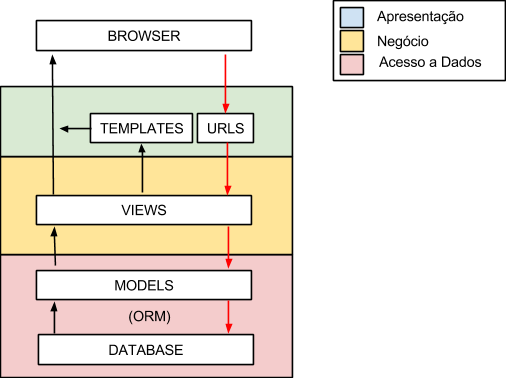
\includegraphics[width=15cm]{figuras/figura_arquitetura.png}
\caption{Desenho Geral da Arquitetura}
\label{figura_arquitetura}
\end{figure}

Nessa arquitetura, o browser do cliente utiliza de uma URL para realizar uma 
requisição numa view, essa view pode utilizar os models para extrair dados do 
banco de dados e ela própria criar um template ela mesma retornar como uma forma 
de resposta ao usuário, ou então ela pode utilizar um template pronto apenas 
moldar esses dados dentro de um template pronto e retornar isso ao browser do 
cliente. 

\section{Padrões de projeto}
Um padrão de projeto representa o trabalho de uma pessoa que encontrou o mesmo 
problema, tentou muitas soluções possíveis, selecionou e descreveu uma das 
melhores e você deve se aproveitar disso.

O conhecimento de padrões permite decidir o que deve ser feito e o que deve ser 
evitado, sistemas baseados em padrões têm mais qualidade. Para o AskMath, forma 
analisados alguns padrões  de projeto e selecionados aqueles que poderiam ser 
satisfatoriamente aplicados. 

\subsection{Proxy}
Fornecer um substituto ou marcador da localização de outro objeto para controlar 
o acesso a esse objeto, podemos controlar o acesso aos métodos de uma entidade 
da seguinte forma: cria se uma classe EntidadeProxy que extende de Entidade, e 
reimplementa cada um dos métodos, nessa nova implementação, você solicitar que o 
usuário informe uma autenticação que possua acesso, ao informar, esse método ira 
apenas chamar o método da Entidade.   

\subsection{Chain of Responsibility}
Evitar o acoplamento do remetente de uma solicitação ao seu receptor, ao dar a 
mais de um objeto a oportunidade de tratar a solicitação. Encadear os objetos 
receptores, passando a solicitação ao longo da cadeia até que um objeto a trate.

\section{Objetivos e Restrições Arquiteturas}

Apresentaremos aqui os requisitos e objetivos do software que têm algum impacto 
na arquitetura, tais como: segurança, proteção de dados, privacidade, 
portabilidade, distribuição, reuso. Também são descritos nesta seção restrições 
arquiteturais que se aplicam ao projeto, tais  como:  estratégias  de  modelagem 
 e  implementação,  ferramentas  de  desenvolvimento, sistemas legados. 

\subsection{Requisitos básicos}
\begin{alineascomponto}
	\item Ubuntu Server como sistema operacional de produção.
	\item Utilização apenas de componentes opensource.
	\item PostgresSQL como sistema de gerenciamento de banco de dados.
	\item Django como framework de desenvolvimento.	
	\item O sistema devera ser Web.
\end{alineascomponto}

\subsection{Estratégias de implementação}
\begin{alineascomponto}
	\item Persistência de tipagem (ex: formato de CPF, Data) devem ser feitos 
tanto no cliente através de Javascript, como no servidor através de 
regex(Regular Expression).
	\item Persistência de obrigatoriedade, verificar se todos os campos 
obrigatórios foram  preenchidos deve ser feito tanto no cliente via javascript 
como no servidor e nas duas opções deve-se apresentar alertas caso algum campo 
seja enviado vazio para a requisição.
    
\end{alineascomponto}
